%------------------------------------------------------------
%------------------------------------------------------------
\section{Le langage {\UTP}}
\label{sec:langage-utp}
Le langage {\UTP} décompose la représentation d'une instance 
en 3 composantes : le modèle d'entités, l'ensemble de règles et la solution.
Nous en donnons ici une description informelle. %et
%présentons le catalogue de prédicats,
%le format des règles et des sélecteurs 
%ainsi que leur interprétation sous forme de contraintes. 
Une spécification formelle est présentée dans \cite{uspPATAT22},
et \cite{uspSite}
détaille la syntaxe {\XML} et le format {\JSON} des instances {\UTP}
et donne aussi accès aux codes sources des modèles {\MINIZINC} et {\CHRPP}, aux outils, et à un benchmark d'instances.

%------------------------------------------------------------
%------------------------------------------------------------
\subsection{Modèle d'entités}
\label{sec:entity-model}
Le modèle d'entités d'une instance {\UTP}  est schématisé en Figure~\ref{fig:utp-entity-model}. 
%\corentin{remplacer le schéma de la figure 3 par celui de PATAT => à propager dans APIA aussi}
Il définit l'horizon de temps, la structure
des cours, l'ensemble des ressources, ainsi que des propriétés d'entités et des relations associatives.
L'horizon de temps se décompose en un nombre de semaines, de journées hebdomadaires et de créneaux quotidiens qui sont propres à chaque instance.
%Les semaines partagent les mêmes jours et les jours les mêmes créneaux.
La décomposition des semaines en journées et celle des journées en créneaux quotidiens sont uniformes.
Les semaines et jours se succédant sur l'horizon de temps ne sont pas supposés consécutifs alors que les créneaux quotidiens le sont.
Ces derniers sont de durée égale et divisent la journée de 24h, p. ex., %si la journée se divise en 24 créneaux, ils seront d'une heure chacun. %; 
si elle se divise en 1440 créneaux, 
ils seront d'1 minute chacun.
Les créneaux servent d'unité de temps pour dater démarrage et fin de séances et pour mesurer durées de séance, temps de déplacement entre salles et délais entre séances.

% % For one-column wide figures use
% \begin{figure}[h]
% % \includegraphics{utp-time-grid.eps}
% \caption{{\UTP} 3-layered time grid}
% \label{fig:utp-time-grid}
% \end{figure}

% For one-column wide figures use
\begin{figure*}[ht]
\centering
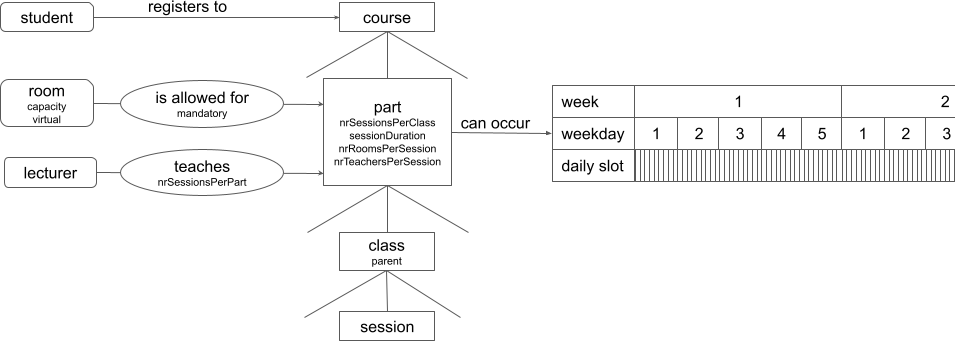
\includegraphics[width=.85\textwidth]{img/utp_entity_model.png}
\caption{Modèle d'entités}
\label{fig:utp-entity-model}
\end{figure*}

Les cours ont une structure arborescente, chaque cours (p. ex. Algo) se décomposant en parties de cours (p. ex. TP d'Algo), chaque partie de cours en classes (p. ex. Classe 2 de TP d'Algo) et chaque classe en séances pré-ordonnées (p. ex. 3\up{ème} séance de la Classe 2 de TP d'Algo).
Les séances sont les tâches élémentaires à ordonnancer quand on résoud une instance {\UTP}, leur nombre, durée et séquencement intra-classe étant fixés.
%Although this approach forbids variable class decompositions, 
%it provides flexibility for handling sessions independently wrt. scheduling and resource allocation.
Précisément, les classes d'une partie de cours comportent un nombre identique de séances de même durée, ces deux constantes étant propres à chaque partie de cours.
%
%Fixed decompositions also facilitates the formulation of requirements which can rely on clear-cut sessions (e.g., planning parallel sessions mid-way through a course, alternating sequences of lecture and practical work sessions).
%
%Les décompositions de manière fixe permettent de faciliter les formulations%TODO
%des besoins%TODO
%en s'appuyant sur un découpages claire des sessions (e.g., planification en parallèle des sessions en milieu de période, faire une alternance entre cours magistraux et travaux pratiques). 
%
%Second, sessions are considered uninterruptible and, in particular, may not overlap two days. 
%Lastly, the schema requires that the sessions of a class be ranked in the entity model and sequenced accordingly in any solution.
D'autre part, le langage impose que les séances d'une classe soient séquencées dans toute solution selon le rang qui leur est associé dans la classe.
Enfin, les séances sont non-interruptibles et en particulier, ne peuvent pas être à cheval sur deux journées.

% % For one-column wide figures use
% \begin{figure}[h]
% % \includegraphics{utp-course-structure.eps}
% \caption{{\UTP} course structure}
% \label{fig:utp-course-structure}
% \end{figure}

%Les ressources{\UTP} fall into 4 types, namely, rooms, teachers, students and (student) groups.
%All the resources of an instance, except groups (see Section~\ref{sec:solutions}), are declared and typed in the entity model.

Trois types de ressources sont modélisés : les salles, les enseignants et les étudiants (constitués en groupes).
Toutes les ressources d'une instance sont déclarées et typées dans le modèle d'entités.
%
%In practice, various restrictions resulting from upstream processes apply on the resourcing and timing of courses (e.g., faculties prescribing degree-specific time grids, departments implementing room pooling policies, alternative candidates designated for teaching courses, students registering for courses).
%
Dans la pratique, différentes contraintes émises en amont s'appliquent aux ressources et aux créneaux de cours (p. ex., facultés imposant une grille horaire par type de cursus, départements mettant en œuvre des politiques de mise en commun de salles, étudiants s'inscrivant aux cours).
%
%Basic restrictions come in the form of compatibility constraints that list the suitable rooms, eligible teachers, candidate students and allowed times for the different courses.
%Such constraints are built in the entity model but scoped differently depending on resource types.
%
Les contraintes les plus élémentaires sont des contraintes de compatibilité énumèrant %liste
les salles appropriées, les enseignants éligibles, les étudiants candidats et les horaires autorisés pour les différents cours.
%
%Precisely, each course part is assigned sets of possible start times, rooms and teachers that are enforced on all its sessions.
Précisément, à chaque partie de cours est assigné l'ensemble des créneaux de départ, de salles et d'enseignants qui sont autorisés pour toutes les séances de la partie (cf. Figure~\ref{fig:utp-entity-model}).
%
%As for students, course registrations are listed separately and %the possible students for a session are those registered to the course it sits in.
%any student registered to a course is considered a possible candidate for each of its sessions.
%Pour les étudiants, l'inscription en cours se fait via une liste qui répertorie tous les cours séparément et tous les étudiants inscrits à un cours sont considéré comme candidat éligible pour chacune de ses sessions.
Concernant les étudiants, l'inscription se fait au niveau des cours, un étudiant devant participer à toutes les parties d'un cours.
La constitution des groupes d'étudiants s'effectue à la résolution du problème ou peut être fournie dans la composante solution. % décrite plus bas.

%Beyond plain compatibility constraints, resource utilization is also subject to demand and capacity constraints.

%Au-delà des simples contraintes de compatibilité, 
L'utilisation des ressources est également soumise à des contraintes de demande et de capacité.
%
%
%Since modalities differ from one environment to the next, the schema supports both disjunctive and cumulative resources as well single- and multi-resource course sessions. 
Comme les modalités diffèrent d'un environnement à un autre, le langage prend en charge les ressources disjonctives et cumulatives ainsi que les séances à ressources uniques ou multiples. 
%
%Students, groups, teachers or rooms qualify as cumulative resources if they 
%can attend, teach or host simultaneous sessions. %, respectively.
Étudiants, enseignants et salles sont qualifiés de ressource cumulative s'ils peuvent suivre, enseigner ou héberger des séances en parallèle.
%
%Cumulative resources are paramount to address flexible attendance requirements (e.g., students assigned optional tutoring sessions that may overlap with mandatory courses) or to handle multi-class events (e.g., rooms hosting joint exam or conference sessions).
Les ressources cumulatives sont indispensables à la modélisation de cours non-obligatoires (p. ex. séances de tutorat facultatives pouvant chevaucher des cours obligatoires) et pour gérer des événements multi-classes (p. ex. salles hébergeant des examens mutualisés).
%
%The schema assumes no limit on the number of parallel sessions teachers and students may attend.
%Rooms however may only host class sessions whose cumulated headcount
%is within their capacity.
Le langage n'impose aucune limite sur le nombre de séances simultanées auxquelles participent enseignants et étudiants.
À l'inverse, les salles ne peuvent héberger que des séances dont l'effectif cumulé est en deça de leur capacité.
%
%Upper bounds on room capacity and class headcounts are encoded for all rooms and classes in the entity model with the possibility to leave room capacity unbounded (e.g., virtual rooms). 
%Note that all resources default to cumulative resources in an entity model and disjunctive behaviour has to be explicitly enforced through rules.
La capacité des salles et les seuils d'effectif des classes sont encodés dans le modèle d'entités qui autorise par ailleurs des salles à capacité illimitée (p. ex. salles virtuelles).
%
Notons que toute ressource est supposée cumulative par défaut
mais des règles disjonctives peuvent être imposées par ressource ou par classe de ressources.
%
%Sessions qualify as multi-resources if they can be allocated multiple resources of the same type at any point in time.

Les séances sont dites multi-ressources si on peut leur allouer plusieurs ressources du même type.
%
%The need for sessions requiring multiple rooms or teachers arises in many practical situations (e.g., multi-room sessions for hybrid teaching, joint supervision of practical work sessions, exams requiring several adjudicators).
Ce type de séances présente un intérêt pratique (p. ex. séances multi-salles pour enseignement hybride, 
séances de travaux pratiques supervisées par plusieurs enseignants, 
examens nécessitant plusieurs surveillants)
et des contraintes s'appliquent alors aux volumes de ressources requis par séance.
Ces dernières s'expriment dans le modèle par des contraintes de cardinalité déclarées sur les parties de cours, chaque partie indiquant le nombre d'enseignants requis par séance (potentiellement aucun) et s'il s'agit de séances à salle unique ou non (\texttt{nrRoomsPerSession} et \texttt{nrTeachersPerSession} en Figure~\ref{fig:utp-entity-model}).
À noter qu'une instance peut mixer des séances
mono-ressource %avec des resoources uniques  
et multi-ressources
et des ressources disjonctives et cumulatives.

Le modèle d'entités incorpore également des contraintes de flot qui
régissent %controle
la distribution des étudiants et des enseignants sur les cours.
Ces contraintes 
sont habituellement émises en amont de la génération d'emplois du temps
durant les phases d'inscription %TODO
et 
de planification de capacité %TODO
(p. ex. distribution des volumes horaires entre enseignants d'un département).
Comme mentionné précédemment, les étudiants s'inscrivent uniquement aux cours. %et non pas aux parties, classes ou séances de cours. 
Résoudre une instance {\UTP} implique donc de placer les étudiants dans les classes conformément à la structure des cours et aux inscriptions demandées.
%
%The implicit rule endorsed in the schema is that a student should be assigned a single class in each part of a course he has registered to and attend all sessions of the selected classes.
La règle adoptée est qu'un étudiant soit assigné à toutes les séances d'une seule classe dans chaque partie de cours.
%
%Group nesting constraints may also be explicitly encoded between classes to enforce equality or set inclusion relations between their sets of participants.
Des contraintes d'imbrication de groupes
peuvent être posées entre classes 
(p. ex. aggréger des groupes de travaux pratiques pour constituer un groupe de cours magistral, préserver les mêmes groupes entre différents cours d'un cursus).
%
%As for staff planning, each teacher is assigned a fixed volume of sessions in each course part it is eligible for, leaving teacher-to-session assignment decisions to solvers.
Pour l'emploi du temps du personnel, chaque enseignant a un volume fixe de séances dans les parties de cours où il intervient, l'affectation des séances restant à déterminer par le solveur.
%
%In addition to built-in types, the schema provides the ability to freely label entities in order to create custom types. 
En complément des types d'entités prédéfinis, le langage offre %permet
la possibilité d'étiqueter
librement les entités du modèle. % afin de créer des types particuliers%personaliser
%
%Precisely, entities sharing the same label in the entity model form a type of their own named after the label.
Les entités qui partagent la même étiquette forment un type à part entière. % nommé d'après cette étiquette.
%
%Labels complement the built-in types and both are used as a means to select entities within rules.
Ces étiquettes peuvent être utilisées à l'instar des types prédéfinis pour sélectionner les entités dans les règles.

%------------------------------------------------------------
%------------------------------------------------------------
\subsection{Ensemble de règles}

\begin{table*}[ht]
%\resizebox{\textwidth}{!}{%
\small
\centering
\begin{tabular}{|l|l|l|p{.6\textwidth}|}
\hline
\textbf{Nom}               & \textbf{Arité} & \textbf{Paramétrique} & \textbf{Sémantique}\\ \hline

%assign\_slot               & 1         & yes   & Assign a slot or slot tuple to a session\\ \hline
%assign\_room               & 1         & yes   & Assign a set of room to session in entry\\ \hline

%allocation\_group           & 1        & no    & Domain allocation for class with group in the solution\\ \hline
%part\_schedule              & 1        & no    & Allowed start time slots for sessions\\ \hline
%domain\_class\_group        & 1        & no    & Allowed groups for classes (solution input)\\ \hline
%domain\_session\_teacher    & 1        & no    & Allowed teachers for sessions\\ \hline
%domain\_class\_room         & 1        & no    & Allowed rooms for sessions\\ \hline

{\SAMEDAILYSLOT}            & 1         & non    & Les séances démarrent le même créneau quotidien\\ \hline
{\SAMEWEEKDAY}              & 1         & non    & Les séances démarrent la même jour de la semaine\\ \hline
{\SAMEWEEKLYSLOT}           & 1         & non    & Les séances démarrent les mêmes créneau et journée\\ \hline
{\SAMEWEEK}                 & 1         & non    & Les séances démarrent la même semaine\\ \hline
{\SAMEDAY}                  & 1         & non    & Les séances démarrent le même jour\\ \hline
{\SAMESLOT}                 & 1         & non    & Les séances démarrent en même temps\\ \hline
{\FORBIDDENPERIOD}          & 1         & oui   & Les séances ne peuvent pas débuter dans la période donnée\\ \hline
{\ATMOSTDAILY}              & 1         & oui   & Le nombre de séances dans la période journalière définie est limité\\ \hline
{\ATMOSTWEEKLY}             & 1         & oui   & Le nombre de séances dans la période hebdomadaire définie est limité\\ \hline
%implicit\_sequenced\_sessions & 1 & \multicolumn{4}{|c|}{no} & All sessions in classes are sequenced\\ \hline
{\SEQUENCED}                & $\geq2$   & non    & Les séances sont séquencées\\ \hline
{\WEEKLY}                   & 1         & non    & Les séances démarrent les mêmes créneaux et jours de semaines successives \\ \hline

{\NOOVERLAP}                & 1         & non    & Les séances ne peuvent être en parallèle\\ \hline
{\TRAVEL}                   & 1         & oui   & Définition du temps de trajet entre salles\\ \hline

{\SAMEROOMS}                & 1         & non    & Les séances ont lieu dans les mêmes salles\\ \hline
{\SAMESTUDENTS}             & 1         & non    & Les mêmes étudiants suivent les séances\\ \hline
{\SAMETEACHERS}             & 1         & non    & Les séances sont encadrées par les mêmes enseignants\\ \hline

{\ADJACENTROOMS}            & 1         & oui   & Les séances doivent être dans des salles adjacentes\\ \hline

{\TEACHERDISTRIBUTION}      & $\geq2$   & oui   & Distribue la charge des enseignants dans les classes\\ \hline

\end{tabular}
%}
\caption{Catalogue des prédicats {\UTP}}
\label{tab:catalogue_predicats}
\end{table*}

Les règles sont utilisées pour formuler des conjonctions de contraintes.
Il s'agit de pouvoir exprimer, de manière concise, une ou plusieurs contraintes liées à un même prédicat.
L'expression d'une règle implique d'identifier l'ensemble des séances que l'on souhaite contraindre et de choisir le prédicat à appliquer.
La table~\ref{tab:catalogue_predicats} liste les prédicats \UTP{} actuellement implémentés et utilisés dans nos instances.

Une règle porte, selon l'arité de son prédicat, sur un ou plusieurs domaines d'e-maps qui associent chacune une entité à un ensemble de séances compatibles.
Les domaines d'e-maps ne sont pas représentés en extension mais à l'aide de sélecteurs. 
Un sélecteur permet de cibler des entités selon leur type, leur étiquette ou leur identifiant et de filtrer les ensembles de séances associées selon leurs rangs et leur compatibilité avec d'autres entités.
%Un sélecteur permet ainsi de réduire l'ensemble de toutes les séances à un sous-ensemble selon si les séances sont liées à une entité spécifique (un élément de cours comme une partie, ou une ressource comme un enseignant), et en fonction de leur rang (pour sélectionner la $n$-ième séance).
%Un sélecteur combine un générateur et une liste optionnelle de filtres.
%Les filtres et le générateur s'expriment de la même manière, le générateur permettant d'indiquer comment les séances doivent être regroupées.
%L'ensemble des séances d'un sélecteur est l'intersection des ensembles de séances du générateur et éventuellement des filtres.
%L'ensemble des séances de la règle est le produit cartésien des ensembles de séances définis par les sélecteurs.
Une règle se traduit ensuite par la conjonction de contraintes obtenue en instanciant le prédicat sur le produit cartésien des domaines d'e-maps sélectionnées.
%Lorsque le type du générateur ou du filtre est une ressource, alors la contrainte générée par la règle ne s'appliquera qu'aux séances réellement associées à la ressource.
%
%Generators and filters are triples 
%$
%(T_i,L_i,O_i)
%$
%consisting of
%an entity type
%$
%T_i%\in{\TYPE}
%$,
%an entity label or identifier
%$
%L_i%\in{\LABEL}
%$
%and
%a subset of session ranks
%$
%O_i%\subseteq{\RANK}
%$ (a.k.a., session mask),
%the latter two elements being optional.
%A selector 
%matches any e-map
%whose entity satisfies the type, label and identifier constraints of the generator
%and whose %set of sessions 
%image includes any compatible session
%satisfying the mask of the generator
%and one of the filters.
%Note that rules featuring empty selectors are discarded during the flattening stage. 
%%Selectors are encoded as attributes in the {\XML} language
%%using a syntax that borrows from the CSS selector language.
%%For instance, the above example would be encoded by the following XML fragment: 
%%\todo[inline]{Marc : Rajouter une phrase pour décrire brièvement la figure 3}

\begin{figure*}[h]
\centering
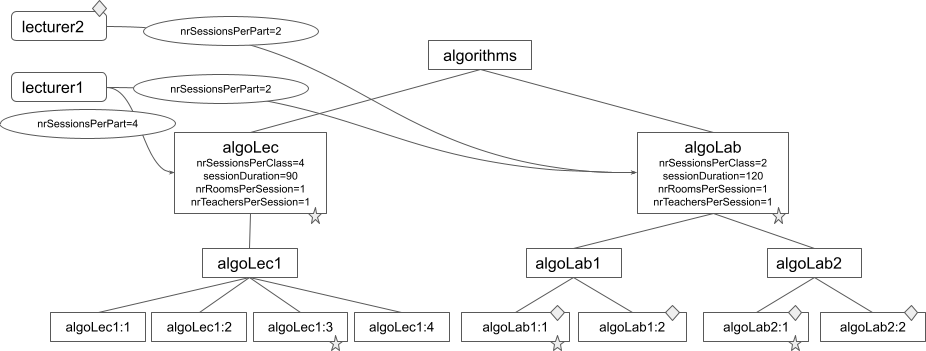
\includegraphics[scale=.45]{img/utp_rule_1.png}

%{\small{
%\begin{flalign}
%&\texttt{{\FORBIDDENPERIOD}((<(\TEACHER,{teacher2},\_)>,9120,9240)}
%&\label{rule-example-1}
%\\
%&\texttt{{\SEQUENCED}(<(\CLASS,\_,\myset{3}),(\PART,{algoLec},\_)>}
%\texttt{\mbox{<(\CLASS,\_,\myset{1}),(\PART,{algoPra},\_)>)}}
%&\label{rule-example-2}
%\end{flalign}
%}}
\newcounter{save_equation}
\setcounter{save_equation}{\value{equation}}
\setcounter{equation}{0}

\renewcommand{\theequation}{R\arabic{equation}}

{\footnotesize{
\begin{flalign}
&\texttt{{\SEQUENCED}(<(\CLASS,\_,\myset{3}),(\PART,{algoLec},\_)>,
<(\CLASS,\_,\myset{1}),(\PART,{algoLab},\_)>)}
&\label{rule-example-1}
\\
&\texttt{{\FORBIDDENPERIOD}((<(\TEACHER,{lecturer2},\_)>,9120,9240)}
&\label{rule-example-2}
\end{flalign}
}}


\setcounter{equation}{0}
\renewcommand{\theequation}{C\arabic{equation}}

%
{
\footnotesize
\begin{flalign}
&\texttt{{\SEQUENCED}((algoLec1,\{algoLec1:3\}), (algoLab1,\{algoLab1:1\}))}
&\label{constraint-example-1}
\\
&\texttt{{\SEQUENCED}((algoLec1,\{algoLec1:3\}), (algoLab2,\{algoLab2:1\})}
&\label{constraint-example-2}
\\
&\texttt{{\FORBIDDENPERIOD}((lecturer2,\{algoLab1:1,algoLab1:2,algoLab2:1,algoLab2:2\}),9120,9240)}
&\label{constraint-example-3}
\end{flalign}
}
%

\caption{Sélection de séances par des règles}
\label{fig:utp-rule-1}
\end{figure*}

%Figure~\ref{fig:utp-rule-1} illustrates the rules flattening process on a small example.
%Course \texttt{algorithmic} is split into a lecture part \texttt{algoLec} and a practice part \texttt{algoPra}.
%The lecture part has a single class of 4 sessions taught by \texttt{teacher1} and the practice part has 2 classes of 2 sessions each taught by \texttt{teacher1} or \texttt{teacher2}.
%%Figure~\ref{fig:utp-rule-1} illustrates the flattening of the following rules: 
%%on a simple model consisting of 2 teachers and & course subdivided into 2 parts, 3 classes and 8 sessions. The first rule forbids a time period for 
%Rule~(\ref{rule-example-1}) below requires that teacher \texttt{teacher2} have no session between $9120$ and $9240$, that is, between 8am and 10am on Tuesday of week 2. 
%%In this rule, $9120$ (resp. $9240$) is the value\footnote{Each possible session schedule is mapped to a single value. All possible values make up the domain of a session.} that corresponds to 8am on Tuesday (resp. 10am on Tuesday) of week 2. 
%The selector includes no mask and no filter hence matches with all possible sessions of \texttt{teacher2} as indicated with diamonds on Figure~\ref{fig:utp-rule-1}. 
%The resulting domain of e-maps is the singleton $\myset{(teacher2,\map{\TEACHER}{\SESSION}{teacher2})}$ and the rule is flattened into a single \texttt{\FORBIDDENPERIOD} constraint. %%$\myset{\map{\TEACHER}{\SESSION}{teacher2}}$.
%Rule~(\ref{rule-example-2})
%%requires that the first practical session in Algorithmic \todo[inline]{Marc : pourquoi algo ?} start after the third lecture.
%requires that the first sessions of the practices start after the third lecture.
%The two selectors include a filter. The first selector matches with all class sessions of rank 3 in part \texttt{algoLec}, and the second matches with all class sessions of rank 1 in part \texttt{algoPra} as indicated with stars on the figure.
%The rule is flattened into 2 \texttt{\SEQUENCED} constraints corresponding to the cross product of the e-map domains $\myset{(algoLec1,\map{\RANK}{\SESSION}{3}\cap\map{\PART}{\SESSION}{algoLec})}$ and $\myset{(algoPra1,\map{\RANK}{\SESSION}{1}\cap\map{\PART}{\SESSION}{algoPra}),(algoPra2,\map{\RANK}{\SESSION}{1}\cap\map{\PART}{\SESSION}{algoPra})}$.


La Figure~\ref{fig:utp-rule-1} illustre la sélection de séances sur un exemple jouet et la génération automatique de contraintes à partir de deux règles.
Le cours \texttt{algorithms} est divisé en une partie de cours magistraux \texttt{algoLec} et une partie de travaux pratiques \texttt{algoLab}.
Le cours magistral est dispensé par \texttt{lecturer1} et ne contient qu'une classe de 4 séances. Les travaux pratiques sont encadrés par \texttt{lecturer1} et \texttt{lecturer2}, et sont constitués de 2 classes de 2 séances.

La première règle (\ref{rule-example-1}) %Deux règles sont illustrées : % en Figure~\ref{fig:utp-rule-1}
stipule que les travaux pratiques de chaque classe ne peuvent commencer qu'après la troisième séance de cours magistral (entités et séances annotées avec une étoile).
Elle est associée au prédicat \texttt{\SEQUENCED} et utilise deux sélecteurs : le premier sélectionne la troisième séance de la partie \texttt{algoLec}, le second sélectionne, pour chaque classe, les premières séances de la partie \texttt{algoLab}.
La partie \texttt{algoLab} ayant deux classes, la règle produit deux contraintes liées à \texttt{\SEQUENCED} : la première (\ref{constraint-example-1}) avec les séances \texttt{algoLec1:3} et \texttt{algoLab1:1}, la seconde (\ref{constraint-example-2}) avec les séances \texttt{algoLec1:3} et \texttt{algoLab2:1}.

La seconde règle (\ref{rule-example-2}) stipule que \texttt{lecturer2} est indisponible sur une période donnée (losanges).
Elle est associée au prédicat \texttt{\FORBIDDENPERIOD} et utilise un sélecteur qui cible les séances de l'enseignant \texttt{lecturer2}.
La règle produit une seule contrainte (\ref{constraint-example-3}) liée à \texttt{\FORBIDDENPERIOD} (avec les paramètres spécifiant la période d'absence de l'enseignant, ici la période entre les créneaux 9120 et 9240) portant sur l'ensemble des séances de la partie \texttt{algoLab} où peut intervenir \texttt{lecturer2}.
La contrainte ne sera effective que sur deux de ces séances étant donné que \texttt{lecturer2} encadre deux séances de travaux pratiques ; ces séances seront identifiées pendant la résolution.




%------------------------------------------------------------
%------------------------------------------------------------
\subsection{Solution}
%The solution component includes assignment decisions relating to the choice of slots and resources for sessions, the placement of students in groups and the assignment of groups to classes.
%The solution hence represented may be partial, see empty, and does not have to be consistent with the built-in constraints or the rules of the instance.
%The support for partial solutions allows to tackle subproblems using separate {\UTP} instances and solution seeds.
%For instance, a scheduling instance may be defined on the basis of partial and consistent solutions pre-generated for the student sectioning and resource allocation subproblems.
%Likewise, the support for inconsistent solutions is paramount to repair solutions that have become inconsistent due to unforeseen changes.
L'élément solution comporte des choix de créneaux et de ressources pour les séances, de groupes pour les étudiants, et de classes pour les groupes.
La solution ainsi représentée peut être partielle, voire vide, et n'est pas nécessairement consistante avec les contraintes de l'instance.
Le support des solutions partielles permet de cibler et résoudre des sous-problèmes. %en utilisant différentes instances \UTP{}.
Par exemple, une instance se réduit à un problème d'ordonnancement si elle se base sur une solution complète pour la constitution des groupes et l'affectation des ressources.
De même, le support des solutions inconsistantes est un pré-requis pour la réparation de solutions qui seraient devenues inconsistantes suite à des changements non-anticipés (p. ex. absence d'un enseignant, indisponibilité d'une salle suite à des travaux).

%%As mentioned before, 
%Student groups are considered a by-product of student sectioning.
%For this reason, groups may only be listed in the solution component, not in the entity model, and defined both by the students they include and the classes they are assigned to. 
%This sectioning process is subject to different constraints. 
%First, groups may only include students with identical course registrations.
%Second, students are inextricably bound to their group, % and indirectly assigned sessions 
%that is, students must be partitioned into groups consistently with their registration profile. %which are given in the entity model.
%Third, group-to-class assignments must comply with any subgroup inclusion constraint stated in the entity model.
Les groupes d'étudiants sont considérés comme le résultat du problème de sectionnement.
Pour cette raison, les groupes font partie de l'élément solution, et définissent à la fois l'ensemble des étudiants qui les composent et les classes auxquelles ils appartiennent.
Ce processus de sectionnement est soumis à différentes contraintes.
D'une part, les groupes ne peuvent être constitués que d'étudiants qui sont inscrits aux mêmes cours.
Ensuite, chaque groupe est insécable sauf dans le cas de séances multi-salles.
Enfin, l'affectation des groupes aux classes doit satisfaire aux contraintes d'inclusion entre classes définies dans le modèle d'entités.








